%===================================== CHAP 4 =================================

\chapter{System Components}
This chapter contains a brief description of the system that has been used.
\section{Hardware}
This section outline the physical components in the x8 and the base station.
\subsection{UAV}\label{ss:SkywalkerX8}
The Skywalker X8, see \ref{figure:skywalkerX8}, is a fixed wing \gls{uav} that is moulded out of \gls{epo}, which makes it a cheap and robust platform for prototype testing. The large space within the fuselage makes it ideal for experimental payload. 
\begin{figure}[H]
	\centering
		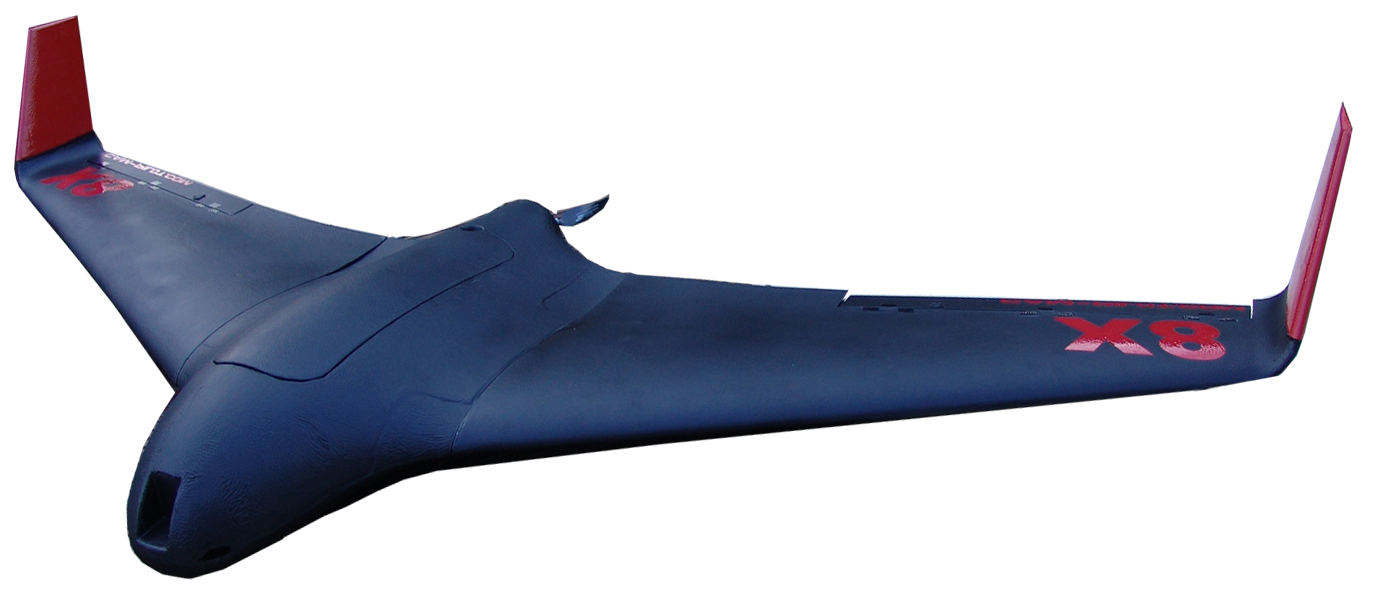
\includegraphics[width=0.7\textwidth]{figs/Wing-X8_white-bgd2.png}
		\caption{X8 Skywalker from Skywalker Technologies, Picture from \url{www.campilot.tv/blog/win-x8}}
		\label{figure:skywalkerX8}
\end{figure}
The X8 has a wingspan of $2120mm$ which allow for \gls{auw} of $3500g$. More specification about the X8 can be found at \citep{hobbyking}. The components that is used in the X8 at the UAVLAB is given in table \ref{tb:X8Components}.
\begin{table}[H]
\begin{center}
\begin{tabular}{l l}
TX & Spektrum DX7s \\
RX & Spektrum Remote Receiver SPM9645 \\
Servo & Hitec HS-5085MG \\
Motor & Hacker A40-12S V2 14-Pole \\
ESC & Master Spin 66 Pro \\
Propeller & Aeronaut 13x8 folding propeller \\
Battery & 1 Zippy Compact 4S 5000 mAh and 1 Haiyin 800 mAh \\
Autopilot & 3D Robotics Pixhawk w/3DR uBlox \gls{gps} with Compass\\& kit and airspeed sensor \\
Telemetry link & 3D Robotics radio (433MHz)
\end{tabular}
\end{center}
\caption{Components in the X8 at the UAVLAB}
\label{tb:X8Components}
\end{table}
\subsection{Embedded Computer}
The embedded computer in the \gls{uav} is a BeagleBone Black
List why this embedded computer is chosen. 

Demands: Must run LSTS in real time, calculate rtkgps wight and size number of output pins.
\begin{figure}[H]
	\centering
		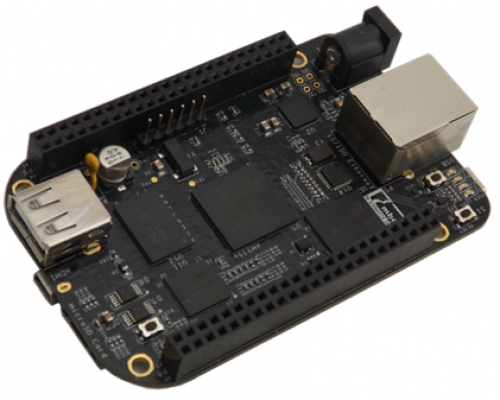
\includegraphics[width=0.7\textwidth]{figs/BeagleBoneBlackE14.png}
		\caption{BeagleBone Black element 14, Picture from \url{http://www.element14.com}}
		\label{figure:BeagleBone}
\end{figure}
\subsection{GNSS receiver}
The system will use two types of \gls{gnss} receivers, namely the Ublox LEA M8T and the Piksi system. 
\subsubsection{Ublox LEA M8T}
The Ublox LEA M8T is a new generation of low-cost \gls{gnss} receiver from ublox. The receiver support sending out raw \gls{gnss} data from both \gls{gps} and \gls{glonass} in the same configuration. The receiver have great performance in acquisition and tracking sensitivity of \gls{gnss} satellites. More technical detalise can be found in  \citep{UbloxDataSheet,UbloxReceiverDescription}.
Write about the Ublox LEA M8T gnss receiver. Also include that it support sending GPS and GLONASS data at the same time. Need to be configured. A receiver were prepare and mounted in the x8.
\begin{figure}[H]
	\centering
		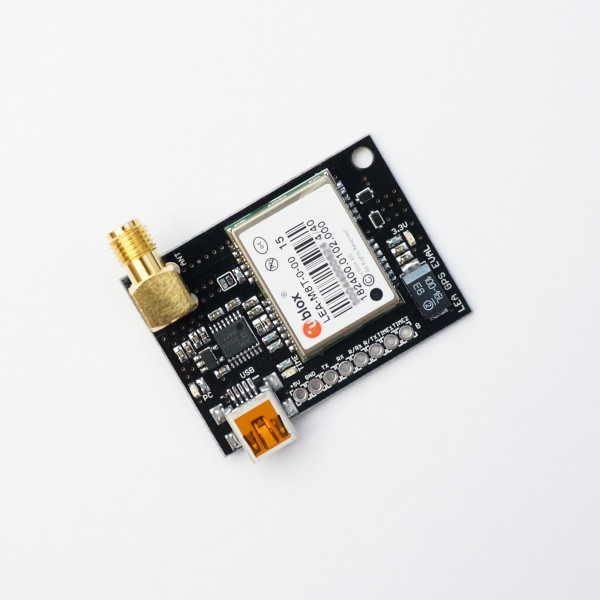
\includegraphics[width=0.7\textwidth]{figs/ubloxLeaM8T.jpg}
		\caption{Ublox LEA M8T, Picture from \url{http://www.csgshop.com}}
		\label{figure:Ublox}
\end{figure}
\subsubsection{Piksi}\label{ss:Piksi}
Piksi, see figure \ref{figure:Piksi}, is a low cost, high performance \gls{gps} receiver with \gls{rtk-gps} functionality with capability for centimeter level relative positioning accuracy developed by Swift Navigation. Piksi is ideal for autonomous vehicles because of its small form factor, fast position solution update rate and low power consumption. 
More detailed information about Piksi can be found in \citep{Piksiv231}
\begin{figure}[H]
	\centering
		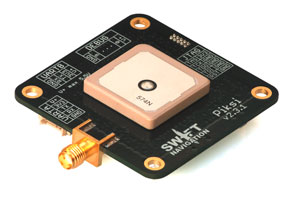
\includegraphics[width=0.7\textwidth]{figs/piksi_top.jpg}
		\caption{Piksi, Picture from \url{www.swiftnav.com}}
		\label{figure:Piksi}
\end{figure}
\section{Software}
This section contain the different software that is used in the x8 system. The following sections contain the operating system that runs on the base station and rover, the middleware used to connect the different tasks, the messages protocol, the missionplaner program and rtklib which will have the main focus.\subsection{GLUED}
Glued is a minimal Linux distribution developed by LSTS, and design with embedded system in mind. It is platform independent, easy to configure and contain only the necessary packages to run on a embedded system. This makes GLUED a light and fast distribution. GLUED is configured through a single configuration file that which can be created for a specific system. 
\subsection{Dune}
Dune is a runtime environment for unmanned systems on-board software created by LSTS (Underwater Systems and Technology Laboratory) in Porto, Portugal. The environment type is called a middleware, which is seeing increase usage in unmanned systems. Can refer to ROS or MOOS middleware.

Dune works by setting up individual task that can dispatch and subscribe to different IMC messages. The IMC messages will be explained in \ref{ss:IMC}
A type of middleware. write how to link rtklib with dune
Refer to the dune wiki page
\subsection{IMC}\label{ss:IMC}
The IMC (write gls here when fixed) protocol that is designed and implemented by LSTS (gls) that is build to interconnect systems of vehicles,sensors and human operators. The protocol is a messages-oriented protocol that enable exchange of real-time information about the environment and updated objectives, such that the participant in the communication can pursue a common goal cooperatively.
IMC has a standard way of dispatching and consuming messages, which abstracts hardware

Other feature: Not assuming a specific software architecture, can generate native support for different programming languages and/or computer architectures. Used in network nodes, inter-process and inter thread communication
\subsection{Netpus}

\subsection{RTKLIB}\label{ss:Rtklib}
Rtklib is a open source program package for standard and precise positioning with GNSS developed by T. Takasu. Rtklib can use raw GNSS data to estimate the position of the rover. Rtklib can be configured to give a position solution in real time in differential mode. Figure \ref{figure:RTKLIB_STRUCTURE} shows how rtklib can be used in a RTKGNSS mode. The two main moduels here is str2str and rtkrcv. Both will be explalined more closely in the following sections. More information about  rtklib can be found in \citep{Rtklib242}.

\begin{figure}[H]
	\centering
		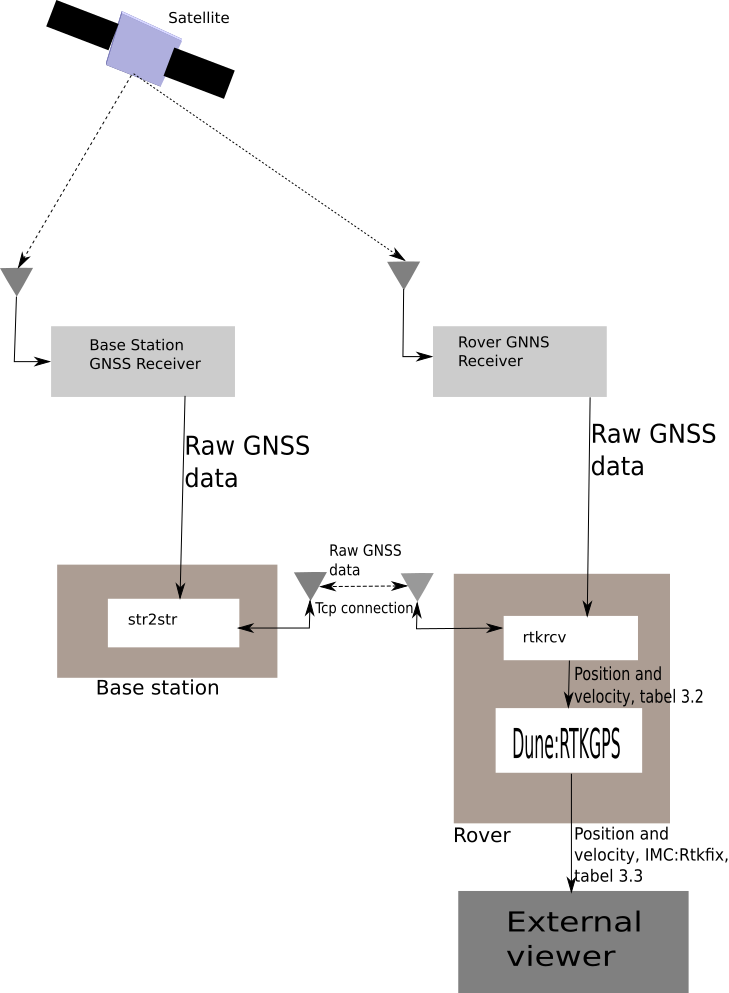
\includegraphics[width=0.7\textwidth]{figs/Rtklib_structure.png}
		\caption{The communication structure of rtklib}
		\label{figure:RTKLIB_STRUCTURE}
\end{figure}
\subsubsection{rtkrcv}
Rtkrcv is the app program that calculate the position of the rover.
Rtkrcv can be configured to have two output streams. The structure of the output stream is given the rtklib manual, however there has been done some alteration in the structure of the output. It's desired in a autonumos landing system that have that velocity solution. This is was not provided in the newest version of rtklib, and therefore the source code was altered to send out the velocity data. A quick note here is that it is only available in the output solution is in a enu format.

When set configured as a differential GPS rtkrcv uses the LAMBDA method to resolve the integer ambiguity. The solution is considered fixed if the ration between the best estimate and the second best estimate is above a certain threshold.
The solution body is given is table 
\begin{table}[!h]
\begin{center}
    \begin{tabular}{ | l | l |}
    \hline
    \textbf{Header} & \textbf{Content} \\ \hline
     1 Time & The epoch time of the solution indicate the true receiver\\& signal reception time. Can have the following format:\\&\\& yyyy/mm/dd HH:MM:SS.SSS:\\& Calender time in GPST, UTC or JST.\\&\\&
     
     WWWW SSSSSSS.SSS:\\&
     GPS week and TOW in seconds  \\ \hline
     2 Receiver Position & The rover receive antenna position \\ \hline
     3 Quality flag (Q) & The flag which indicates the solution quality.\\& 1:Fixed\\& 2:Float\\& 5:Single \\ \hline
     4 Number of valid satellites (ns) & The number of valid satellites for solution estimation. \\ \hline
     5 Standard deviation & The estimated standard deviation of the\\& solution assuming a priori error model and error\\& parameters by the positioning options \\ \hline
     6 Age of differential & The time difference between the observation data epochs\\& of the rover receiver and base station in second. \\ \hline
     7 Ratio factor & The ratio factor of "ratio-test" for standard integer\\& ambiguity validation strategy \\ \hline
     8 Receiver velocity & The velocity of the rover. Given only when output is\\& in enu format \\ \hline
    \end{tabular}
\end{center}
\caption{Table 1. }
\label{Tab1}
\end{table}
The position solution is calculated with a Extended Kalman Filter, that can have different structure depending on how rtkrcv is configured
\subsubsection{str2str}
Str2str is the app program that retrieve the ublox signal from the gps and sends over tcp to the rtkrcv app. The str2str is setup to either send RMTC 3 messages, or whatever is send in from the GPS. Since the str2str do not support to send ublox signal directly. How to write that the user should not specify the input format or the output format.



\cleardoublepage